\documentclass[11pt, preprint]{article}
\usepackage{hyperref}
\usepackage{rotating}
\usepackage[normalem]{ulem}
\usepackage{environ}
\usepackage{xcolor}
\usepackage{amsmath}

 
\setlength{\footnotesep}{9.6pt}
\setlength{\parskip}{12pt}

\newcounter{thefigs}
\newcommand{\fignum}{\arabic{thefigs}}

\newcounter{thetabs}
\newcommand{\tabnum}{\arabic{thetabs}}

\newcounter{address}

\NewEnviron{answer}[1][]{\color{blue}\expandafter\BODY
{\par \it #1}}

\begin{document}

\begin{center}
  {\bf Radiative Processes in Astrophysics / Problem Set \#4 /
    Answers}
\end{center}


\begin{enumerate}
\item The cosmic microwave background at $z\sim 1100$ is the last
  scattering surface of the photons from the hot ionized gas that
  filled the universe before that time. Before recombination, these
  photons Thomson scatter efficiently off the electons in the ionized
  gas, and are kept in thermal equilibrium at about $T\sim 3000$ K at
  that epoch. As hydrogen atoms recombine at $z\sim 1100$, the gas
  becomes transparent to most of these photons, which then travel
  towards us.
\begin{enumerate}
\item Using the known cosmic baryon density, estimate the mean free
  path (in physical units) of a photon to Thomson scattering when the
  ionization fraction is 0.5.

  \begin{answer}
    The number density of electrons in comoving units will be $\sim
    f_i \rho_c \Omega_{b,0} / m_p$, where $f_i$ is ionization
    fraction, $\rho_c$ is the critical density, and $m_p$ is the
    proton mass (neglecting the contribution of helium). At redshift
    $z$, in physical units the density will be higher by a factor
    $(1+z)^3$. The mean free path will be $l = 1/n_e \sigma_T$, or:
    \begin{equation}
      l = \frac{m_p}{(1+z)^3 f_i \rho_c \Omega_{b,0} \sigma_T} \sim
      10^{22} {\rm ~cm} \sim 3 {\rm ~kpc~(physical)}
    \end{equation}
  \end{answer}
\item The photons reaching us are those emitted exactly normal to the
  surface defined by the recombination epoch. These photons are the
  result of scattering from the gas surrounding the point in
  question. If the temperature of the CMB were uniform, do you expect
  the light reaching us to be polarized, and if why or why not?

  \begin{answer}
    Imagine observing a point on the sky.  If the gas there was
    illuminated from just one direction, some of that light would be
    scattered to us.  The maximum polarization case would be if it
    were scattering from a direction perpendicular to our line of
    sight to the point on the sky (i.e. from somewhere in the
    tangent). In that case the linear polarization would be 100\%,
    aligned perendicular to the direction between the light source and
    the point on the sky we are observing. See Figure \ref{fig:pol} to
    illustrate this.
    
    But if the gas at that point on the sky is illuminated 
    uniformly from all directions, as it would be if the temperature
    was uniform, the polarizations would be canceled and the net
    polarization would be zero.
  \end{answer}

      \begin{figure}[h!]
        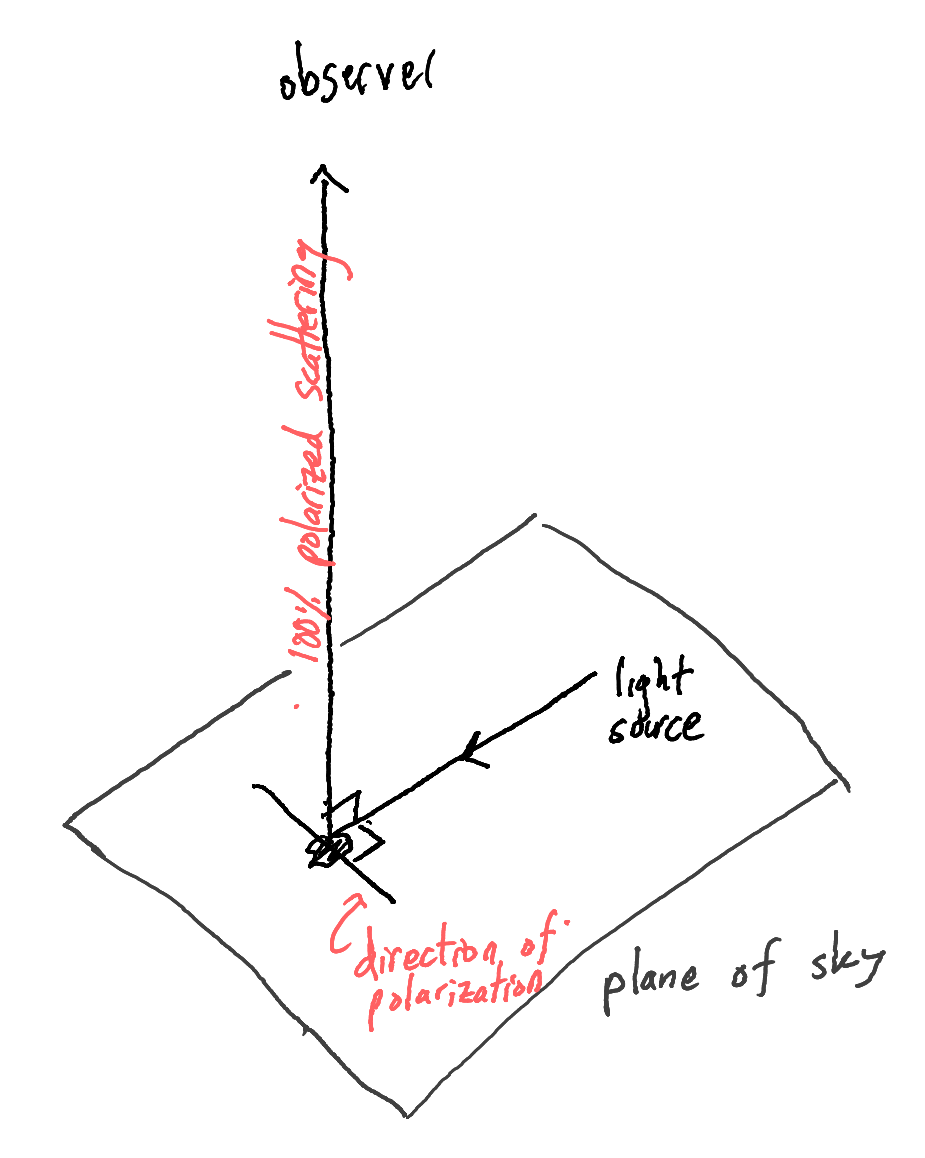
\includegraphics[width=0.9\textwidth]{ans-4-pol.png}
        \caption{ \label{fig:pol} Diagram showing the ray with 100\%
          polarization (normal to illumination direction) from Thomson
          scattering and the direction of polarization (normal to
          illumination direction {\it and} that ray). }
      \end{figure}
      \clearpage
      
\item Considering a local patch of the reionization surface, sketch a
  pattern of temperature fluctuations on the surface that would yield
  a net polarization.

\begin{answer}
  A quadrupolar pattern of temperature (e.g. as in Figure
  \ref{fig:quad}), higher towards left and right on the page, colder
  towards up and down on the page, will lead to a net
  polarization. Light coming from the up and down directions causes
  polarized scattering in the left-right direction. However, the light
  from the left and right directions causes polarized scattering in
  the up-down direction.  If the intensity of light were the same in
  all directions (e.g. part (b)) then the net polarization would be
  zero. But if the left and right directions are hotter on average
  than the up and down directions, then they contribute more
  intensity, and (as shown) a net polarization in the up-down
  direction remains.
\end{answer}

      \begin{figure}[h!]
        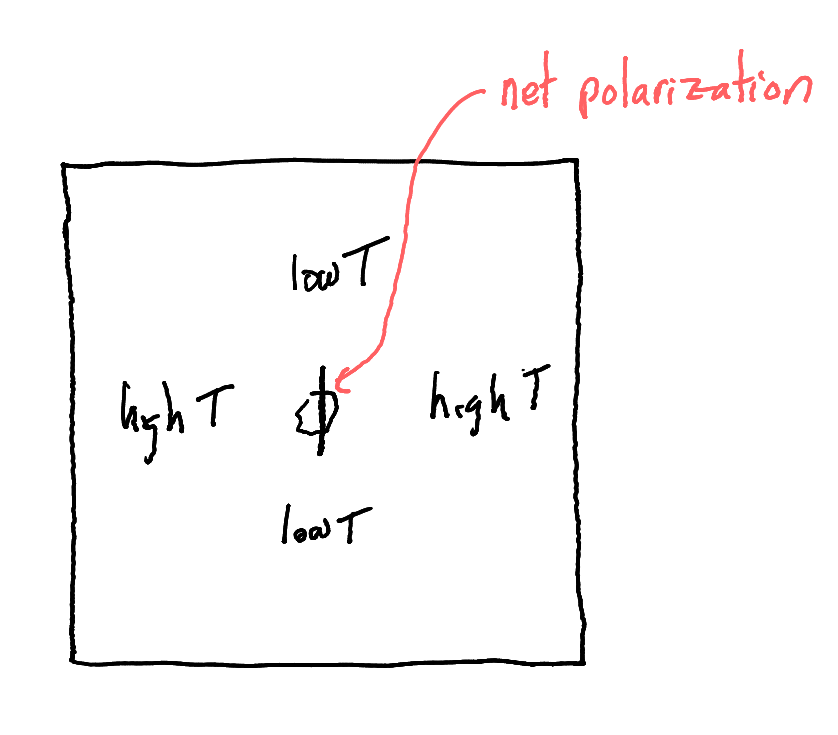
\includegraphics[width=0.9\textwidth]{ans-4-quad.png}
        \caption{ \label{fig:quad} Diagram showing a distribution on
          the plane of the sky of CMB temperatures that would result
          in net polarization, along with the direction of the
          polarization.}
      \end{figure}
\end{enumerate}

\item Consider the dependence of the ``equivalent width'' associated
  with an absorption line with a Voigt profile, on the optical depth
  at line center. Assumed the absorbed continuum is flat in
  $f_\lambda$. You may treat ${\rm d}\lambda/\lambda \propto {\rm
    d}\nu/\nu$ in the region of the line. The equivalent width is the
  integral of the absorbed light in $f_\lambda$ divided by the flux
  density of the continuum in $f_\lambda$. The dependence of EW on
  $\tau$ is called the ``curve-of-growth.''
  \begin{enumerate}
    \item For $\tau\ll 1$, approximate the dependence of equivalent
      width on $\tau$. 

      \begin{answer}
        If we take a constant continuum $I_{\nu, 0}$ in the absence of
        absorption, the equivalent width can be written as:
        \begin{equation}
          \mathrm{EW} = \frac{\lambda_0^2}{c} \frac{\int {\rm d}\nu (I_{\nu,0} -
            I_\nu)}{I_{\nu,0}} = \frac{\lambda_0^2}{c} \int {\rm d}\nu
          \left[1 - \exp(-\tau_\nu)\right]
        \end{equation}

        If the optical depth at line center $\tau\ll 1$, then we can
        expand the exponential and obtain:
        \begin{equation}
          \mathrm{EW} = 
            \frac{\lambda_0^2}{c} \int {\rm d}\nu
          \tau_\nu
        \end{equation}

        We can write:
        \begin{equation}
          \tau_\nu = \tau \phi(\nu)
        \end{equation}
        where $\phi$ is defined to be unitless and to be unity at
        $\nu=\nu_0$. $\phi(\nu)$ is remaining fixed so:
        \begin{equation}
          \mathrm{EW} = 
            \frac{\lambda_0^2}{c} \tau \int {\rm d}\nu
          \phi(\nu) \propto \tau
        \end{equation}
      \end{answer}
    \item For $\tau\gg 1$, neglecting the Lorentzian term
      (i.e. $\Gamma = 0$), approximate the dependence of equivalent
      width on $\tau$.

      \begin{answer}
        In this case, we can write:
        \begin{equation}
          \mathrm{EW} = \frac{\lambda_0^2}{c} \int {\rm d}\nu
          \left[1 - \exp\left(-\tau \phi(\nu)\right)\right]
        \end{equation}
        Consider the spectral region around the line, with the offset
        from the line $\Delta\nu = \nu - \nu_0$. If $\tau\gg 1$, then
        the integrand is unity until $\phi(\Delta\nu) \sim 1/\tau$,
        and then it quickly transitions to zero. In  this case, we
        refer to the center of the line as {\it saturated}---i.e. the
        absorption is completely obliterating the light.

        Thus:
        \begin{equation}
          \mathrm{EW} \sim \frac{\lambda_0^2}{c}
          \int_{-\Delta\nu}^{\Delta\nu} {\rm d}\nu \sim \frac{2
            \lambda_0^2}{c} \Delta\nu
        \end{equation}
        For a Gaussian $\phi(\nu)$ we can find where its value is
        $1/\tau$:
        \begin{eqnarray}
          \exp\left[-\Delta \nu^2 / 2\sigma_\nu^2\right] &=&
          \frac{1}{\tau} \cr
          \Delta \nu &=& \sigma_\nu \sqrt{2 \ln \tau}
        \end{eqnarray}
        From which we find:
        \begin{equation}
          \mathrm{EW} 
          \sim \frac{2
            \lambda_0^2}{c} \sigma_\nu \sqrt{2 \ln \tau}
        \end{equation}
      \end{answer}
    \item For $\tau\gg 1$, neglecting the Doppler term
      (i.e. $\sigma = 0$), approximate the dependence of equivalent
      width on $\tau$.

      \begin{answer}
        In this case, the line profile is (recalling we are
        normalizing so $\phi(\nu_0) = 1$):
        \begin{equation}
          \phi = \frac{(\Gamma / 4\pi)^2}{\left(\nu - \nu_0\right)^2 +
            \left(\Gamma / 4\pi\right)^2}
        \end{equation}
        Solving for the $\Delta \nu$ for which $\phi = 1/\tau$ we find:
        \begin{equation}
          \Delta \nu = \frac{\Gamma}{4\pi} \sqrt{\tau -
            1}
        \end{equation}
        which leads to (for $\tau\gg 1$):
        \begin{equation}
          \mathrm{EW} 
          \sim \frac{2
            \lambda_0^2}{c} 
          \frac{\Gamma}{4\pi} \sqrt{\tau}
        \end{equation}
        Note that the prefactor here about a factor of two too small,
        because unlike the Gaussian the Lorentzian doesn't fall off
        too quickly.
      \end{answer}
    \item Assume $\Lambda$ is the classical damping width, and the
      velocity dispersion $\sigma =$ 10 km s$^{-1}$. Based on the
      scalings you just calculated, sketch (the log of) equivalent
      width vs $\tau$.

      \begin{answer}
        At low $\tau$ the EW will scale linearly, and then it will
        transition as the line saturates in its center.  At very high
        $\tau$ the tails of the Lorentzian wings will dominate
        (because $\sqrt{\tau}$ rises much more quickly than $\sqrt{\ln
          \tau}$).

        If the Gaussian is much narrower than the Lorentzian, then the
        convolution with the Gaussian doesn't really affect the EW
        curve of growth, so it would look like just a transition near
        $\tau \sim 1$ from linear to square-root dependence.

        But if the Lorentzian is narrower than the Gaussian, then as
        $\tau$ rises, there will be a regime where the center is
        saturated but the overall width is dominated by the
        Gaussian. Only at higher $\tau$ will the $\sqrt{\tau}$ scaling
        from the Lorentzian wings catch up with the $\sqrt{\ln \tau}$ scaling
        of the Gaussian.

        So which situation are we in? We have to choose a wavelength
        regime to consider. Recall from the calculation of $\Gamma$:
        \begin{equation}
          \Gamma = \left(\frac{2e^2}{3c^3 m}\right) (2\pi)^2 \nu_0^2
          \sim \left(4 \times 10^{-22} \mathrm{~s}\right) \nu_0^2
        \end{equation}
        For $\lambda_0 \sim 6000$ \AA we have:
        \begin{equation}
          \nu_0 = \frac{c}{\lambda_0} \approx 0.5 \times 10^{15}
          \mathrm{~s}^{-1}
        \end{equation}
        and then for the Lorentzian its FWHM is $\Gamma \sim 10^8$
        s$^{-1}$.

        For the Gaussian, its FWHM will be $\sim 2.35 \sigma_\nu \sim
        2.35 \nu_0 \sigma /c \sim 3\times 10^{10}$ s$^{-1}$.

        Therefore in this case the Lorentzian core is much narrower
        than the Gaussian, and the curve-of-growth will have a phase
        with a $\ln \tau$ dependence.

        So the EW will rise linearly with $\tau$, almost plateau with
        $\sqrt{\ln \tau}$, and then start to rise as $\sqrt{\tau}$.
      \end{answer}
  \end{enumerate}
  
\end{enumerate}

\end{document}

